% Sablon pentru realizarea lucrarii de licenta, conform cu recomandarile
% din ghidul de redactare:
% - https://fmi.unibuc.ro/finalizare-studii/
% - https://drive.google.com/file/d/1xj9kZZgTkcKMJkMLRuoYRgLQ1O8CX0mv/view

% Multumiri lui Gabriel Majeri, acest sablon a fost creat pe baza
% codului sursa a lucrarii sale de licenta. 
% Codul sursa: https://github.com/GabrielMajeri/bachelors-thesis
% Website: https://www.gabrielmajeri.ro/
%
% Aceast sablon este licentiat sub Creative Commons Attribution 4.0 International License.

\documentclass[12pt, a4paper]{article}

% Setează fontul Times
\usepackage{times}

% Modificarea geometriei paginii (Margini setate la 2.5cm)
\usepackage[margin=2.5cm]{geometry}

% Setează spațiere inter-linie la dublu
\usepackage{setspace}
\doublespacing

% Utilizează biblatex pentru referințe bibliografice
\usepackage[
    backend=biber,
    maxbibnames=50,
    sorting=nty
]{biblatex}
\addbibresource{refs.bib}

% Include funcțiile de grafică
\usepackage{graphicx}
% Încarcă imaginile din directorul `images`
\graphicspath{{../images/}}

% Listări de cod
\usepackage{listings}

% Linkuri interactive în PDF
\usepackage[
    colorlinks,
    linkcolor={black},
    menucolor={black},
    citecolor={black},
    urlcolor={blue}
]{hyperref}

% Comenzi matematice
\usepackage{amsmath}
\usepackage{mathtools}
\usepackage[
    warnings-off={mathtools-colon,mathtools-overbracket}
]{unicode-math}

% Formule matematice
\newcommand{\bigO}[1]{\symcal{O}\left(#1\right)}
\DeclarePairedDelimiter\abs{\lvert}{\rvert}

% Suport pentru anexe
\usepackage{appendix}
\usepackage{titlesec}
\usepackage{float}

\titleformat{\chapter}
  {\normalfont\LARGE\bfseries}
  {\thechapter.}
  {0.5em}
  {}

% Metadate
\title{A Post-hoc Interpretability Analysis of xLSTM
Architectures}
\author{Tănase Victor-Flavian}

% Generează variabilele cu @
\makeatletter
\let\ps@plain\ps@empty
\makeatother

\begin{document}

% Front matter
\cleardoublepage

% Pagina de titlu
\begin{titlepage}

% Redu marginile
\newgeometry{left=2cm,right=2cm,bottom=1cm}

\begin{figure}[!htb]
    \centering
    \begin{minipage}{0.2\textwidth}
        
\includegraphics[width=\linewidth]{logo-ub.png}
    \end{minipage}
    \begin{minipage}{0.5\textwidth}
        \large
        \vspace{0.2cm}
        \begin{center}
            \textbf{UNIVERSITY OF BUCHAREST}
        \end{center}
        \vspace{0.3cm}
        \begin{center}
            \textbf{
                FACULTY OF \\
                MATHEMATICS AND COMPUTER SCIENCE
            }
        \end{center}
    \end{minipage}
    \begin{minipage}{0.2\textwidth}
        
\includegraphics[width=\linewidth]{logo-fmi.png}
    \end{minipage}
\end{figure}

\begin{center}
\textbf{SPECIALIZATION ARTIFICIAL INTELLIGENCE}
\end{center}

\vspace{1cm}

\begin{center}
\Large \textbf{Master Thesis}
\end{center}

\begin{center}
\huge \textbf{\MakeUppercase{A Post-hoc Interpretability Analysis of xLSTM
Architectures}}
\end{center}

\vspace{3cm}

\begin{center}
\large \textbf{GRADUATE}\\[0.5em]
\large \textbf{Tănase Victor-Flavian}
\end{center}

\vspace{0.25cm}

\begin{center}
\large \textbf{SCIENTFIC COORDINATOR \\ Cristian Rusu PhD}
\end{center}

\vspace{2cm}

\begin{center}
\Large \textbf{Bucharest, July 2026}
\end{center}
\end{titlepage}
% \include{Title-ro}
\restoregeometry
\newgeometry{
    margin=2.5cm
}
\addtocounter{page}{1}

% Rezumatul
\begin{center}
{\Large \textbf{Abstract}}
\end{center}
Recent progress in natural language processing has been largely driven by large language models(LLMs).
These architectures aim to learn representations of text that capture syntax, 
semantics, and long-range dependencies in an efficient and scalable way. 
Despite significant advances in performance, the internal mechanisms by which these models store and manipulate information 
remain only partially understood. \\ \\
% 
This limitation becomes especially relevant in deep models that rely on fundamentally 
different approaches to information storage. Transformer-based models process sequences using 
self-attention, where information is mixed across tokens at each layer without an explicit notion 
of persistent memory. In contrast, the xLSTM, a recently developed architecture was proposed 
by Beck et al. \cite{beck2024xlstmextendedlongshortterm} as an alternative to the transformer architectures 
by extending the classic LSTM cell and reviving the interest in Recurrent Neural Networks \\ \\ 
%
This work performs an analysis of the xLSTM architecture through a set of interpretability 
experiments aimed at understanding how information is represented, stored, and transformed inside the 
model. Moreover, the practicality of this architecture is assessed by evaluating it in a question answering 
setup, a very common application of LLMs. \\ \\ 
%
We track how the model's intermediate hidden states evolve and compare them to those produced by a Transformer model
to assess the similarity of their internal representations. 
Furthermore, we inspect memory behavior during the processing of sequences to understand how individual tokens influence 
the retention and discarding information. \\ \\
%
Finally, we evaluate memory caching as a practical use of xLSTM's fixed-size memory state. By reusing the memory 
state after processing the context, the model avoids recomputing the input sequence and achieves inference 
speedups that increase with context length. We compare this approach against Mistral-7B and examine the 
trade-off between inference efficiency and task performance.



\begin{center}
{\Large \textbf{Sinopsis}}
\end{center}
Progresul recent în prelucrarea limbajului natural a fost accelerat de 
dezvoltarea modelelor lingvistice de mari dimensiuni(LLM). Acest tip de arhitectura 
are ca scop învățarea unor reprezentări ale limbajului care pot captura proprietăți 
sintactice, semantice și să învețe relații între cuvinte îndepărtate într-un mod efficient
și scalabil. În ciuda progresului acestor modele, modul în care ele 
învață și manipulează informația este doar parțial înțeles. \\ \\
%
Această limitare este cu atât mai relevantă în arhitecturile profunde care se bazează pe 
abordări diferite de a înmagazina informația. Modelele de tip transformer procesează
secvențe de text cu ajutorul mecanismului de atenție, care folosește informația din tokeni în fiecare
strat intern, fără o structură definită pentru memorie. Pe de altă parte, xLSTM o arhitectură 
recurentă a fost propusă recent de către Beck et al.\cite{beck2024xlstmextendedlongshortterm} ca o 
alternativă la modelele transformer, extinzând versiunea clasică a celulei LSTM. \\ \\
%
Această lucrare propune o analiză a arhitecturii xLSTM printr-un set de experimente menite să 
ajute la înțelegerea felului în care informația este reprezentată, stocată si transformată în cadrul modelului. 
Mai mult, evaluăm practicalittea acestei arhitecturi într-un scenariu de tip
intrebare-raspuns, o utilizare foarte frecventă a modelelor LLM. \\ \\
%
Se propune observarea evoluției reprezentărilor latente intermediare, precum și comparația cu cele produse de 
un model Transformer pentru a evalua similaritatea dintre ele. 
Mai mult, analizăm comportamentul stării de memorie pe parcursul procesării textului pentru a 
înțelege felul în care tokeni individuali influențează adăugarea 
și eliminarea de informație în memorie. \\ \\ 
%
Concluzionând, evaluăm stocarea în cache a stării de memorie a modelului, exploatând dimensiunea
fixă a acesteia. Prin reutilizarea stării de memorie după procesarea contextului, modelul evită reprocesarea contextului
și îmbunătățește viteza de generare a răspunsurilor direct proporțional cu lungimea contextului. 
Această metodă este evaluată în comparație cu utilizarea în aceleași condiții a unui model Mistal-7B cu scopul de a examina
avantajele și dezavantajele privind eficiența inferenței și performanța modelului în cadrul experimentului.

\tableofcontents

% Main matter
\cleardoublepage

\section{Introduction}
\label{ch:introduction}

Since the inception of the Transformer \cite{vaswani2017attention}, large architectures utilizing stacked 
attention mechanisms have dominated the research landscape, exhibiting impressive performance in 
natural language processing tasks. This architectural paradigm scaled rapidly, progressing from hundreds
of millions of parameters to billions, and ultimately to trillions for enterprise-scale models. In parallel, 
with this scaling trend, a significant part of the scientific community focused their efforts on understanding
the internal mechanisms of these models. However, this intense scientific work has focused
almost exclusively towards attention-based architectures, leaving non-transformer based models comparatively less explored. \\ \\
%
Despite their success, Transformers suffer from a fundamental computational bottleneck: the 
self-attention mechanism scales quadratically ($\mathcal{O}(N^2)$) with respect to sequence length, making long-context
processing computationally expensive. This limitation has led to a recent resurgence of interest in recurrent and 
state-based architectures that aim to achieve linear-time efficiency ($\mathcal{O}(N)$) without sacrificing performance. 
Key contributions in this direction include: Structured State Space Models (SSMs) like Mamba \cite{gu2024mambalineartimesequencemodeling}, 
linear transformers such as Receptance Weighted Key Value (RWKV)\cite{peng2023rwkvreinventingrnnstransformer} and 
Extended Long-Short Term Memory(xLSTM) \cite{beck2024xlstmextendedlongshortterm}. \\ \\
%
The xLSTM architecture extends the classic LSTM cell \cite{10.5555/2998981.2999048} by 
introducing exponential gating and matrix-valued memory states with gated updates. These changes look to address the scaling 
problem of the Transformers and the storage bottlenecks of traditional LSTMs, and try to achieve comparable perfromance while 
maintaining linear-time inference.  

\subsection{Problem}

Deep architectures have produced tremendous advancements in the field of machine learning over the past decade. 
Their pattern recognition and information representation capabilities are yet to be completely understood even to this day.
Post-hoc interpretability in deep neural networks is a challenging problem due to several intrinsic mathematical 
and structural properties of these models. \\ \\
%
First, modern architectures operate in high-dimensional representation spaces, 
where features are distributed across multiple dimensions. Moreover, multiple concepts may be encoded within 
overlapping directions of the representation space. \\ \\
%
Second, neural networks apply a sequence of non-linear transformations, making the relationship between input tokens 
and internal representations difficult to describe. As network depth increases, interactions 
between representations become progressively more complex. \\ \\ 
%
Finally, although the computation of hidden states is fully 
specified by the model parameters and architecture, the resulting computation graph is generally too complex to provide 
specific human-interpretable explanations of how particular representations or predictions are produced. \\ \\
%
Beyond interpretability challenges, recurrent-based architectures such as xLSTM also introduce important systems-level 
considerations. In contrast to purely attention-based models, recurrent models maintain an evolving internal state that 
can, in principle, reduce the computational overhead associated with processing long contexts. However, in practice, 
the models suffer from significant generation latency due to the sequential nature of the RNNs. 
This makes efficient inference an important bottleneck to be addressed, particularly when dealing with long sequences or real-time constraints. 

\subsection{Motivation}

The motivation for this work originates from the recent resurgece of recurrent architectures in large-scale sequence 
modelling. While analyizing the current state of research on recurrent neural networks, the xLSTM architecture, which 
Beck et al.\cite{beck2024xlstmextendedlongshortterm} proposed in 2024, became a personal point of interest. As one of the 
first recurrent architectures in recent years to demonstrate competitive performance at scales traditionally 
dominated by Transformer-based models, xLSTM represents an important development in the ongoing search for efficient 
alternatives to self-attention. \\ \\ 
%
While the performance of Transformer-based language models has been extensively studied, a substantial body of 
interpretability research has also emerged to investigate their internal mechanisms. In contrast, the behavior 
of modern recurrent architectures such as xLSTM remains comparatively underexplored. This observation motivated 
the present work, which applies and adapt interpretability techniques inspired by previous studies of 
neural language models. \\ \\
%
By investigating how information is represented, stored, and updated within xLSTM, this thesis aims to contribute 
to a better understanding of the model's memory mechanisms and internal representations. Such insights may help 
validate architectural design choices, identify limitations, and inform future developments of memory-based language models.\\ \\
%
At the same time, it is important to evaluate how alternative architectures perform in practice compared to Transformers, 
which are widely used and benefit from highly optimized inference systems. This motivates the study of xLSTM under realistic 
inference conditions.
\subsection{Contribution}

To address the lack of interpretability analyses for scalable recurrent architectures, the main objective of this thesis is 
to perform a post-hoc evaluation of the internal representations and state dynamics of the xLSTM-7B architecture. 
This work analyzes the internal mechanisms of the model by first studying the hidden states and then examining the individual components
of the xLSTM cells that contribute to the hiden state values.\\ \\ 
%
The first phase of this work establishes an empirical baseline by evaluating the pretrained xLSTM-7B model across standard 
datasets, specifically LAMBADA (OpenAI)\cite{paperno2016lambada}, 
PIQA\cite{bisk2020piqa}, Winogrande\cite{sakaguchi2021winogrande}, ARC-Challenge\cite{clark2018arc}, ARC-Easy\cite{clark2018arc}, 
and Hellaswag\cite{zellers2019hellaswag}. This evaluation represents an assessment of the model's capablities before 
analyzing its internal structure. Following this initial evaluation, the second phase adapts the logit lens\cite{nostalgebraist2020logitlens}
\cite{belrose2023tunedlens} to project intermediate hidden states from the recurrent layers directly onto the vocabulary space. \\ \\
%
Next, we compare how hidden representations evolve across the layers of a recurrent network compared to a Transformer, 
using xLSTM-7B and Mistral-7B. The final two phases of the interpretability study focus on the sequential processing of the architecture. 
Specifically, we examine the evolution of the memory state over time and the contribution of individual 
tokens to long-term memory through the input and forget gates. To analyze these mechanisms, we process
sequences and track the norm of the cell state, together with the activations of the input and forget gates. 
This allows us to observe how information is stored, retained, and updated throughout the sequence. \\ \\ 
%
On top of the interpretability experiments, we evaluate the practical utility of the xLSTM model in a 
question answering setting. We leverage the constant-size memory state of the model and explore caching 
it when processing context that is later reused for answering questions. This approach enables an inference 
speedup that increases with the size of the context, as the stored memory can be reused without recomputing 
the full sequence.
\subsection{Outline}

This thesis is structured as follows. Section~\ref{ch:related-work} presents the theoretical background underlying the work. It introduces Recurrent Neural Networks, Long Short-Term Memory cells, and the Extended Long Short-Term Memory architecture.
\\ \\ 
Section~\ref{ch:method} describes the methodology used in the experiments. More specifically, it outlines the research objectives, the models considered, and the experimental setup, including the theoretical formulation of the conducted experiments. The technologies and implementation details are presented in Section~\ref{ch:implementation}.
\\ \\
Section~\ref{ch:experiments} presents and discusses the experimental results. Finally, conclusions, limitations, and directions for future work are provided in Section~\ref{ch:conclusion-and-future-work}.
\section{Preliminaries and Related Work}
\label{ch:related-work}

To provide the necessary background for the evaluation of the xLSTM-7B architecture,
this chapter presents the theoretical concepts and related work relevant to this study.
The first section reviews the evolution of recurrent neural networks, from classical RNNs
to the modern architecture proposed by Beck et al. \cite{beck2024xlstmextendedlongshortterm} 
that incorporate gating mechanisms and matrix-based memory structures. \\ \\
%
\subsection{Recurrent Neural Networks}
Recurrent Neural Networks (RNNs) represent one of the earliest neural architectures specifically 
designed for sequence modeling tasks. Their foundations can be traced to the work of Rumelhart et al. 
\cite{rumelhart1986learning}, who introduced the backpropagation algorithm and discussed neural networks 
with recurrent connections. Unlike feedforward neural networks, which process each input independently, 
RNNs maintain a hidden state that evolves over time, allowing information from previous inputs to influence 
future predictions. \\ \\
%
The key idea behind recurrent architectures is the reuse of the same set of parameters at every time step. 
Given an input sequence, the hidden state is updated recursively based on both the current input and the 
previous hidden state, enabling the network to capture temporal dependencies within the data. This property 
made RNNs a natural choice for tasks involving sequential information, such as language modeling, speech 
recognition, machine translation, and time-series forecasting.

\begin{figure}[htbp]
    \centering
    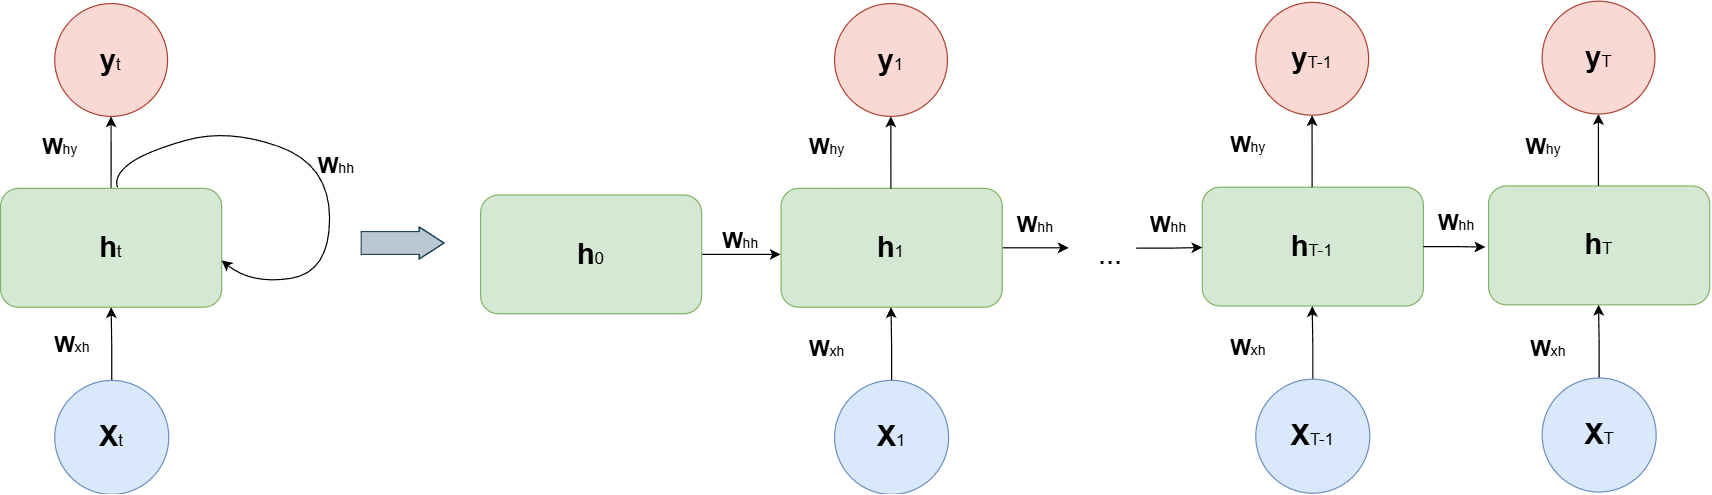
\includegraphics[width=\textwidth]{RNN.png}
    \caption{RNN: compressed (left) and unfolded(right), diagram inspired by \cite{olah2015lstm}}
    \label{fig:RNN-diagram}
\end{figure}
\noindent The operation of a standard RNN can be formally described through its hidden state update (equation \ref{eq:vanilla-rnn-equation}).
At a given timestamp $t = \overline{1, T}$, for an input $x_t$, the hidden state $h_t$ is computed as: 
\begin{equation}
h_t = \phi(W_{xh}x_t + W_{hh}h_{t-1} + b_h),
\label{eq:vanilla-rnn-equation}
\end{equation}

where $W_{xh}$ and $W_{hh}$ are learnable weight matrices, $b_h$ is a bias term, and $\phi(\cdot)$ 
denotes a non-linear activation function such as $\tanh$ or sigmoid. The hidden state is then used to 
produce the output $y_t$: 

\begin{equation}
y_t = W_{hy}h_t + b_y,
\label{eq:y_t RNN}
\end{equation}

where $W_{hy}$ and $b_y$ are the output weight matrix and bias, respectively. Through the recurrent 
connection involving $h_{t-1}$, the network is able to propagate information across time steps, 
allowing previous inputs to influence future predictions.\\ \\ 
%
Training recurrent neural networks requires propagating gradients not only through the layers of the network but also 
through time. This is typically achieved using \textit{Backpropagation Through Time} (BPTT), 
introduced by Werbos et al.\cite{werbos1990backpropagation}. BPTT unfolds the recurrent network across the input sequence, 
transforming it into an equivalent deep feedforward network with shared parameters at each time step. Gradients
are then computed by applying the backpropagation algorithm to the unfolded computational graph and accumulated 
across all time steps before updating the model parameters. \\ \\ 
%
While this training procedure allows RNNs to learn temporal dependencies, it also exposes a major limitation of the 
architecture. During BPTT, gradients are propagated backward through all previous time steps of the sequence. 
At each step, the gradient is repeatedly multiplied by the same recurrent transformation, as it is passed through the 
unfolded network in time. As a result, the gradient magnitude may gradually decrease or increase with each multiplication.
When it becomes too small, the network struggles to learn from earlier time steps, a phenomenon known as the \textit{vanishing gradient problem}. 
Conversely, when it grows too large, training becomes unstable, leading to the \textit{exploding gradient problem} \cite{bengio1994learning}.\\ \\ 
%
These issues significantly limit the ability of standard RNNs to capture long-range dependencies in sequential data. 
To address the exploding gradient problem, Pascanu et al. \cite{pascanu2013difficulty} introduced \textit{gradient clipping}, 
a technique that limits the magnitude of gradients during training and improves optimization stability. Nevertheless, 
the difficulty of preserving information over long sequences remained a fundamental challenge, motivating the development 
of more advanced recurrent architectures such as Long Short-Term Memory (LSTM)\cite{10.5555/2998981.2999048} networks 
and Gated Recurrent Units (GRUs)\cite{cho2014learningphraserepresentationsusing}\cite{chung2014empiricalevaluationgatedrecurrent}.

\subsection{Long-Short Term Memory}

The \textbf{Long Short-Term Memory (LSTM)} architecture, introduced by Hochreiter and Schmidhuber \cite{10.5555/2998981.2999048} in the 1990s,
was proposed to address the limitations of standard RNNs when learning long-range dependencies. The key innovation of the architecture is the 
introduction of a dedicated memory state that can preserve information across many time steps. Instead of relying solely on the hidden state, 
the LSTM uses a set of gating mechanisms to control how information is written to, stored in, and retrieved from memory. 
This allows the model to memorize relevant information over longer sequences while reducing the impact of the vanishing gradient problem 
encountered in traditional recurrent networks. \\ \\
%
\begin{figure}[h!]
    \centering
    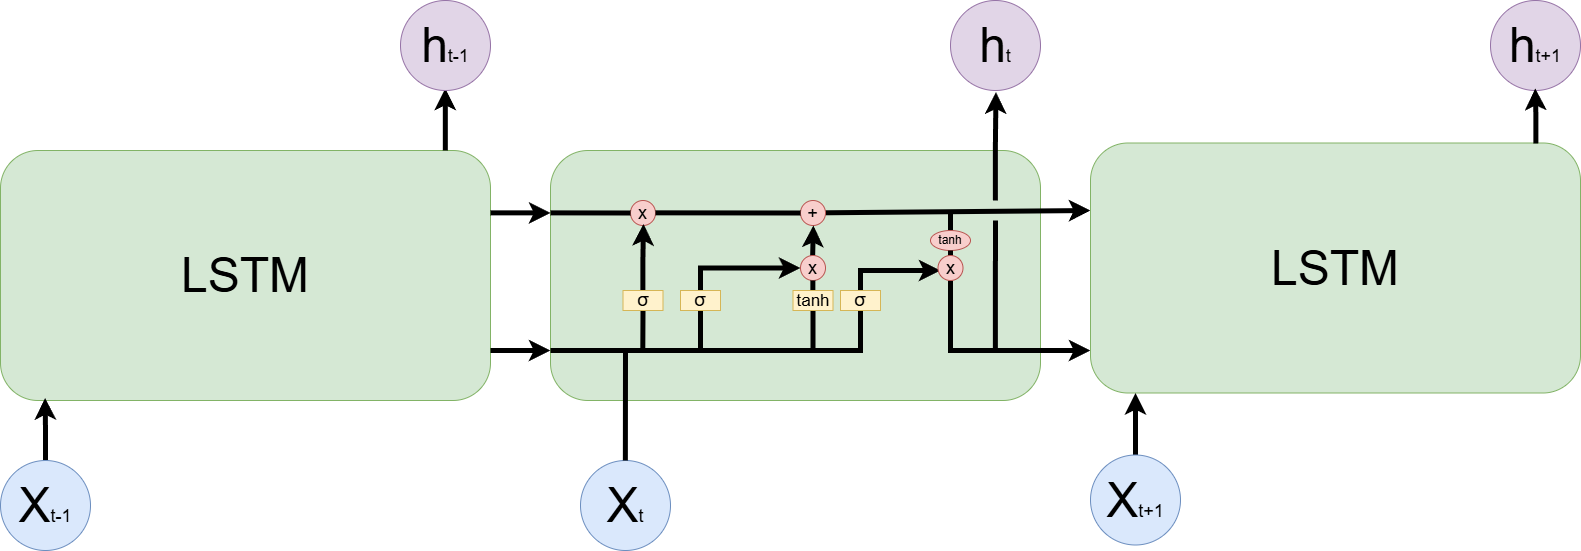
\includegraphics[width=\textwidth]{LSTM.png}
    \caption{The LSTM cell, figure inspired by \cite{olah2015lstm}}
    \label{fig:LSTM}
\end{figure}

\noindent The standard LSTM cell maintains an internal cell state, $c_t$(\ref{eq:lstm_cell_state}), which acts as a long-term memory buffer, 
and a hidden state, $h_t$(\ref{eq:lstm_hidden_state}), 
which serves as the short-term working memory routed to subsequent layers. The flow of information inside the cell is controlled by 
three gates with different scopes. The forget gate(\ref{eq:lstm_forget_gate}) manages what proportion of the historical cell state to discard by analyzing the 
current input and the previous hidden state. The input gate(\ref{eq:lstm_input_gate}) controls how much new information, computed from the current input and 
previous hidden state, is incorporated into the cell state. Finally, the output gate(\ref{eq:lstm_output_gate}) determines which information stored in the 
updated cell state is propagated as the next hidden state.

\begin{equation}
f_t = \sigma(W_f x_t + R_f h_{t-1} + b_f)
\label{eq:lstm_forget_gate}
\end{equation}

\begin{equation}
i_t = \sigma(W_i x_t + R_i h_{t-1} + b_i)
\label{eq:lstm_input_gate}
\end{equation}

\begin{equation}
\tilde{c}_t = \tanh(W_c x_t + R_c h{t-1} + b_c)
\label{eq:lstm_candidate_state}
\end{equation}

\begin{equation}
c_t = f_t \odot c_{t-1} + i_t \odot \tilde{c}_t
\label{eq:lstm_cell_state}
\end{equation}

\begin{equation}
o_t = \sigma(W_o x_t + R_o h_{t-1} + b_o)
\label{eq:lstm_output_gate}
\end{equation}

\begin{equation}
h_t = o_t \odot \tanh(c_t)
\label{eq:lstm_hidden_state}
\end{equation}

\noindent Overall, the introduction of a dedicated memory cell and gating mechanisms 
allows LSTMs to address the limitations of standard RNNs in capturing long-range dependencies. 
However, the sequential processing over the time dimension still limits parallelization and makes them 
computationally expensive for long sequences. Several architectural extensions were later 
proposed to improve their effectiveness in different settings. Bidirectional recurrent networks \cite{schuster1997bidirectional} 
improved contextual understanding by processing sequences in both forward and backward directions,
while encoder-decoder architectures \cite{sutskever2014sequence} enabled sequence-to-sequence learning by separating the encoding 
and decoding processes.
In addition, stacked recurrent architectures \cite{graves2013generating} increased model capacity 
by composing multiple recurrent layers, allowing for more expressive hierarchical representations.\\ \\ 
%
Despite these improvements, these variants did not remove the fundamental sequential bottleneck of recurrent 
computation, which limited scalability on long sequences. These limitations motivated the transition toward 
architectures that avoid recurrence entirely, most notably Transformer\cite{vaswani2017attention} models based on self-attention. 
In this broader context, recent work has revisited recurrent memory mechanisms at scale, leading to 
architectures such as xLSTM, which aim to combine the efficiency of structured recurrence with improved 
scalability and expressive memory modeling. \\ \\ 

\subsection{Extended Long-Short Term Memory}

The extended LSTM (xLSTM) architecture was introduced by Beck et al. \cite{beck2024xlstmextendedlongshortterm} 
to overcome these bottlenecks by leveraging modern techniques 
while fundamentally modifying the LSTM memory structure. 

\subsubsection{Addressing Classic LSTM Limitations}
To understand the architectural shifts in the xLSTM, it is necessary to outline the 
three main bottlenecks of the classic LSTM:
\begin{enumerate}
    \item \textbf{Inability to revise storage decisions:} Traditional LSTMs struggle to
    update or revise a stored value when new, more relevant information is found. 
    %
    \item \textbf{Limited storage capacities:} Information in a classic LSTM is compressed 
    into a scalar cell state, leading to poor performance when predicting rare tokens or 
    retaining extensive context.
    %
    \item \textbf{Lack of parallelizability:} The recurrent memory update relies on hidden-to-hidden 
    connections between consecutive time steps, requiring strictly sequential processing and 
    preventing the highly parallel computation that characterizes Transformer architectures.
\end{enumerate}

\noindent To address these issues, xLSTM introduces several changes to the classical LSTM architecture.
First, it replaces the traditional logistic gating mechanism with \textit{exponential gating}, 
which provides a less restricted range for controlling memory updates. To ensure numerical stability 
during training and inference, xLSTM uses normalization and 
stabilization techniques. In addition, the architecture looks to improve the design of the memory state, 
resulting in two distinct recurrent building blocks: the \textit{scalar LSTM (sLSTM)} and the 
\textit{matrix LSTM (mLSTM)}. While sLSTM extends the traditional LSTM memory formulation with 
improved gating and memory management, mLSTM introduces a matrix-based memory structure capable of 
storing richer associations between tokens.

\subsubsection{sLSTM}
The sLSTM (scalar LSTM) remains structurally closer to the classic architecture but 
introduces exponential activation functions for the input and forget gates. 
This modification allows the model to control its storage more effectively:

% Ensure you have \usepackage{amsmath} and \usepackage{bm} in your preamble
\begin{align}
    \mathbf{c}_t &= \mathbf{f}_t \odot \mathbf{c}_{t-1} + \mathbf{i}_t \odot \mathbf{z}_t && && \text{cell state} \\
    \mathbf{h}_t &= \mathbf{o}_t \odot \tilde{\mathbf{h}}_t, & \tilde{\mathbf{h}}_t &= \psi(\mathbf{c}_t) && \text{hidden state} \\
    \mathbf{z}_t &= \varphi(\tilde{\mathbf{z}}_t), & \tilde{\mathbf{z}}_t &= \boldsymbol{W}_z \boldsymbol{x}_t + \boldsymbol{R}_z \boldsymbol{h}_{t-1} + \boldsymbol{b}_z && \text{cell input} \\
    \mathbf{i}_t &= \sigma(\tilde{\mathbf{i}}_t), & \tilde{\mathbf{i}}_t &= \boldsymbol{W}_{\mathbf{i}} \boldsymbol{x}_t + \boldsymbol{R}_{\mathbf{i}} \boldsymbol{h}_{t-1} + \boldsymbol{b}_{\mathbf{i}} && \text{input gate} \\
    \mathbf{f}_t &= \sigma(\tilde{\mathbf{f}}_t), & \tilde{\mathbf{f}}_t &= \boldsymbol{W}_{\mathbf{f}} \boldsymbol{x}_t + \boldsymbol{R}_{\mathbf{f}} \boldsymbol{h}_{t-1} + \boldsymbol{b}_{\mathbf{f}} && \text{forget gate} \\
    \mathbf{o}_t &= \sigma(\tilde{\mathbf{o}}_t), & \tilde{\mathbf{o}}_t &= \boldsymbol{W}_{\mathbf{o}} \boldsymbol{x}_t + \boldsymbol{R}_{\mathbf{o}} \boldsymbol{h}_{t-1} + \boldsymbol{b}_{\mathbf{o}} && \text{output gate}
\end{align}

\noindent To prevent the numerical overflows specific to the exponential function, a normalizer 
state ($n_t$) and stabilization states are utilised:
\begin{align}
    m_t &= \max \left( \log(f_t) + m_{t-1}, \log(i_t) \right) && \text{stabilizer state} \label{eq:stabilizer-state}\\
    i'_t &= \exp \left( \log(i_t) - m_t \right) = \exp(\tilde{\imath}_t - m_t) && \text{stabil. input gate} \\
    f'_t &= \exp \left( \log(f_t) + m_{t-1} - m_t \right) && \text{stabil. forget gate}
\end{align}

\noindent Despite these changes, because it retains hidden-hidden recurrent connections, 
the sLSTM doesn't improve the sequential processing bottleneck of the classic LSTM.
For the scope of this work, the architecture used in the experiments solely relies on mLSTM cells. 

\subsubsection{mLSTM}
The mLSTM fundamentally shifts the LSTM paradigm to solve both the storage capacity 
and parallelization bottlenecks. To overcome the limited capacity of scalar states, the mLSTM 
expands the memory cell into a matrix $C \in \mathbb{R}^{d \times d}$ where $d$ represents the embedding dimension of $x_{t}$. Crucially, to achieve 
this efficiency, the mLSTM entirely abandons memory mixing (the hidden-hidden recurrent connections) allowing parallelization. \\ \\ 
%
Relying on Bidirectional Associative Memory (BAM)\cite{kosko1987adaptive} principles and Transformer terminology,
the mLSTM stores information as key-value pairs ($k_t$, $v_t$) using a covariance (outer product) 
update rule, and retrieves it using a query vector ($q_t$). The mLSTM cell also uses the stabilizer state introduced in the sLSTM equations(\ref{eq:stabilizer-state})
%
\begin{align}
    \boldsymbol{C}_t &= \mathrm{f}_t \boldsymbol{C}_{t-1} + \mathrm{i}_t \boldsymbol{v}_t \boldsymbol{k}_t^\top && && \text{cell state} \\
    \boldsymbol{n}_t &= \mathrm{f}_t \boldsymbol{n}_{t-1} + \mathrm{i}_t \boldsymbol{k}_t && && \text{norm. state} \\
    \boldsymbol{h}_t &= \mathbf{o}_t \odot \tilde{\boldsymbol{h}}_t, & \tilde{\boldsymbol{h}}_t &= \boldsymbol{C}_t \boldsymbol{q}_t / \max \left\{ \left| \boldsymbol{n}_t^\top \boldsymbol{q}_t \right|, 1 \right\} && \text{hidden state} \\
    \boldsymbol{q}_t &= \boldsymbol{W}_q \boldsymbol{x}_t + \boldsymbol{b}_q && && \text{query input} \\
    \boldsymbol{k}_t &= \frac{1}{\sqrt{d}} \boldsymbol{W}_k \boldsymbol{x}_t + \boldsymbol{b}_k && && \text{key input} \\
    \boldsymbol{v}_t &= \boldsymbol{W}_v \boldsymbol{x}_t + \boldsymbol{b}_v && && \text{value input} \\
    \mathrm{i'}_t &= \exp(\tilde{i}_t - m_t), & \tilde{i}_t &= \boldsymbol{w}_{\mathrm{i}}^\top \boldsymbol{x}_t + b_{\mathrm{i}} && \text{input gate} \\
    \mathrm{f'}_t &= \exp \left( \log(\sigma(\tilde{f_t})) + m_{t-1} - m_t \right), & \tilde{f}_t &= \boldsymbol{w}_{\mathrm{f}}^\top \boldsymbol{x}_t + b_{\mathrm{f}} && \text{forget gate} \\
    \mathbf{o}_t &= \sigma(\tilde{\mathbf{o}}_t), & \tilde{\mathbf{o}}_t &= \boldsymbol{W}_{\mathbf{o}} \boldsymbol{x}_t + \boldsymbol{b}_{\mathbf{o}} && \text{output gate}
\end{align}

\subsection{The xLSTM Block}

The xLSTM block leveages the mLSTM as a multi-head sequence-mixing layer. First, the input token 
representation $x_t$ is normalized with RMSNorm. The normalized vector is then linearly projected into several heads.
Each head receives its own projected query, key, value, and gate information, and each head runs an independent mLSTM cell. 
Therefore, the recurrent state is also stored separately for each head. The outputs of the heads, written as $h_1$, $h_2$, ..., 
$h_N$, are then normalized per head, gated, concatenated, and passed through a shared output linear layer. This produces a vector 
with the same hidden dimension as the original input, so it can be added back through a residual connection. \\ \\ 
%
After the mLSTM sub-layer, the block applies a second pre-RMSNorm residual sub-layer: a SwiGLU feed-forward network. 
This layer does not mix information across time. Instead, it processes each token representation independently. 
The final output of the block is obtained by adding the FFN output back to the result of the mLSTM residual branch. \\ \\
%
\begin{figure}[h!]
    \centering
    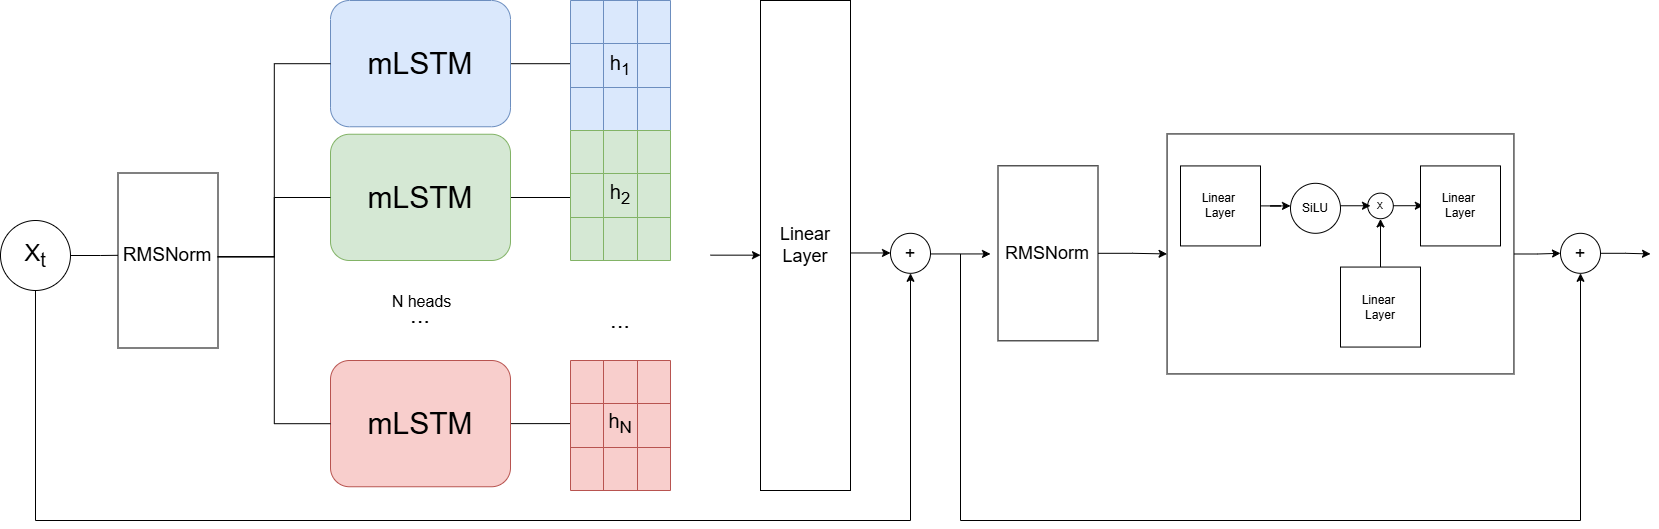
\includegraphics[width=\textwidth]{mlstm-block.drawio.png}
    \caption{mLSTM Block}
    \label{fig:mLSTM-block}
\end{figure}
\noindent This block structure is the one used in the available pre-trained xLSTM-7b model. It differs from the original 
xLSTM paper, where the mLSTM block used a more specialized structure with an up-projection, causal convolution,
block-diagonal query/key projections, and an internal skip connection. In the pre-trained model, the block is 
simpler and closer to a standard transformer block: a multi-head mLSTM sequence-mixing layer followed by a 
SwiGLU feed-forward layer. For the scope of this study, we'll refer to this version of the xLSTM layer.
\section{Method}
\label{ch:method}

\section{Implementation Details}
\label{ch:implementation}

The experiments in this study are implemented in Python using PyTorch and the Hugging Face Transformers library. 
The pretrained weights for both NX-AI/xLSTM-7B and mistralai/Mistral-7B-v0.3 are obtained directly from the Hugging
Face model hub, ensuring a consistent and reproducible experimental setup. \\ \\
%
For benchmark evaluation, we use the LM Evaluation Harness <cite> framework as the primary tool for running standardized model assessments. 
Both this benchmark and the question-answering experiments require multiple inference operations, and for this reason we employ 
NVIDIA A100 GPUs with 40GB and 80GB of memory. The computation is executed in a cloud environment using the Modal infrastructure.\\ \\
%
A significant part of the study relies on accessing internal model representations. For all experiments involving hidden states, 
we employ PyTorch forward hooks to extract intermediate activations during inference. 
This mechanism allows us to capture layer-wise representations without modifying the original model architecture.\\ \\
%
When analyzing the cell states and input/forget gates, these values were not directly 
exposed by the model API. To address this limitation, we reconstruct them by intercepting the hidden states 
before and after each mLSTM block using hooks, and computing the corresponding values using the mathematical 
formulations provided in the xLSTM paper, as well as the reference implementation in the Hugging Face Transformers codebase. \\ \\
%
For the memory caching experiment, we build upon an existing xLSTM caching implementation provided in the model repository
,adapting it to support our experimental setup. This allows us to reuse previously computed memory states during question answering,
reducing redundant computation during inference.
We restrict decoding to a maximum of 25 new tokens and use a temperature of 1.0 
to ensure consistent sampling behavior across runs. The limit of 25 generated tokens is chosen because the SQuAD dataset 
primarily requires short, span-like answers, making longer generations unnecessary for the task. 
Inference time is measured by aggregating per-step execution intervals from the start to the end of generation. \\ \\ 
%
Finally, it is important to note that the xLSTM implementation benefits from optimized custom Triton kernels, 
which provide a significant speedup compared to standard PyTorch kernels. This optimization has a direct impact 
on overall runtime performance across all experiments.
\section{Experiments}
\label{ch:experiments}

\section{Conclusion}
\label{ch:conclusion-and-future-work}
\subsection{General Observations}

Overall, the model shows encouraging learning behavior and seems to be able to process
long contexts efficiently. While its accuracy remains below that of transformer-based
models, it shows a possible advantage in terms to latency and scales well in 
long-context inference scenarios.\\ \\
%
The reproduced benchmark results did not fully match the reported performance, 
likely due to missing implementation details or differences in evaluation frameworks.
This points to a possible sensitivity of reported results to evaluation setup and 
preprocessing choices.
%
Logit lens analysis across stacked recurrent layers reveals behavior similar to transformer 
architectures, where intermediate representations progressively align with final predictions. 
Hidden state comparisons with Mistral-7B showed approximately 95\% CKA similarity in 
the final layers, suggesting that xLSTM develops internal representations closely aligned with those of transformer-based language models. Additionally, the model was able to identify 
and prioritize important tokens within a given sequence, attributing stronger updates to meaningful elements 
such as entities and key contextual markers. The input and forget gates seem to work in a coordinated way to 
preserve relevant information while selectively integrating new content into the memory state. \\ \\
%
Memory caching in a question-answering setup yields up to a 2.7$\times$ speedup in generation 
time by reusing precomputed memory states and avoiding redundant computation over long contexts 
accross 102 question answer pairs.
The speedup increases with context length, making the approach particularly beneficial 
for long-sequence inference. Notably, in our experiments, this improvement was achieved 
\textbf{without any observed degradation in accuracy}. However, performance still remains below 
a comparable transformer baseline (Mistral-7B).
%
\subsection{Limitations}
Despite the promising results, the model underperforms compared to a tranformer similar in size
across several benchmarks. In addition, experimental work was constrained 
by engineering limitations, including difficulties in deploying Triton kernels across 
different operating systems.

\subsection{Future Work}
This study represents an initial exploration of the model's capabilities. Future work should extend
evaluation to longer sequences and include benchmarks that explicitly test long-range memory and 
contextual retention. This would provide a more comprehensive assessment of the model's strengths 
and limitations in long-context reasoning settings.
\newpage
\printbibliography[heading=bibintoc]

\end{document}